\documentclass{article}

\usepackage[margin=2.5cm]{geometry}
\usepackage[pdfauthor = {Tony Mendes},
colorlinks = true,
urlcolor = blue,
linkcolor = blue,
citecolor = blue]{hyperref}
\usepackage{listings, tikz}
\lstset{basicstyle=\ttfamily, frame=single, basewidth=0.5em}

\title{\Huge \LaTeX{} on the Web}
\date{}

\begin{document}

\maketitle

\section{MathJax}

Including mathematics on web pages
with \href{https://www.mathjax.org/}{MathJax} is as easy as including the this
code in the HTML document (usually between \verb~<head>~ and \verb~</head>~ at
the top of the HTML):
\begin{lstlisting}
<script type="text/javascript"
 src="https://cdnjs.cloudflare.com/ajax/libs/mathjax/2.7.5/MathJax.js?config=TeX-AMS_HTML">
</script>
\end{lstlisting}
This code allows mathematics symbols and standard AMS environments (such as
\verb~align~, \verb~bmatrix~, \verb~cases~, etc.) can be typed directly into
the HTML document.  The default settings of MathJax do not interpret dollar
signs as enclosing mathematics, so unless settings are changed then mathematics
must be enclosed within \verb~\(..\)~, \verb~\[..\]~,
\verb~\begin{equation}..\end{equation}~, etc.

Read the documentation at \url{https://docs.mathjax.org/en/latest/index.html}
to discover how to customize MathJax.  One example of such a customization is
the script
\begin{lstlisting}
</script>
<script type="text/x-mathjax-config">
    MathJax.Hub.Config({
	displayAlign: "center",
	displayIndent: "0em",
	"HTML-CSS": { scale: 100,
	              linebreaks: { automatic: "false" },
		      availableFonts: [],
		      webFont: "TeX" },
	SVG: {scale: 100,
	      linebreaks: { automatic: "false" },
	      font: "TeX"},
	NativeMML: {scale: 100},
	TeX: { equationNumbers: {autoNumber: "AMS"},
	       MultLineWidth: "85%",
	       TagSide: "right",
	       TagIndent: ".8em" }});
</script>
\end{lstlisting}
which should appear before the code calling MathJax.

An alternative to MathJax is KaTeX, which claims to have some benefits over
MathJax.  Visit \url{https://katex.org/} for more details.

\section{Exporting to HTML}

A \LaTeX{} file can be converted into HTML (or other file formats) using either
Pandoc or \mbox{LaTeXML}.

Neither one of these tools preserves the font choices called from packages like
\verb~mathspec~ or \verb~fontspec~, so do not load such packages.  Fonts,
colors, and the overall style in HTML is best selected using CSS files after
converted to HTML.

\subsection{Pandoc}

Pandoc is software that converts one markup format to another.  Please visit
\url{https://pandoc.org/} to install.  Read the documentation (or
\verb~man pandoc~ on Linux) to learn how to run pandoc.

If using Linux, a shell command such as
\begin{lstlisting}
pandoc file.tex -f latex -t HTML > file.html
\end{lstlisting}
turns a \LaTeX{} file into an HTML file.  Any mathematics in this HTML file is
kept as LaTeX commands which can then be converted into mathematical symbols
using MathJax.

Pandoc simply interprets the \LaTeX{} document structure as a HTML document
structure.  It does not actually run \LaTeX{} or load any packages.  Therefore
Pandoc does not preserve labels, numbering, and cannot generate graphics with
TikZ.  Pandoc is best for straightforward \LaTeX{} documents.

\subsection{LaTeXML}

LaTeXML is a robust \LaTeX{} converter that attempts to faithfully recreate a
\LaTeX{} document as HTML.  It interacts well with labels, numbering, BibTeX
and TikZ.  Please visit \url{https://dlmf.nist.gov/LaTeXML/} to install.  Read
the documentation (or \verb~man latexml~ and \verb~man latexmlpost~ on Linux)
to learn how to run LaTeXML.

The LaTeXML software converts \LaTeX{} to the XML file format.  Then the XML
file can then be converted to HTML using the latexmlpost command.  For example,
a file can be converted using the shell commands
\begin{lstlisting}
latexml file.tex --destination="file.xml"
latexmlpost file.xml --destination="file.html" --css="file.css"
\end{lstlisting}
The optional \verb~--css="file.css"~ allows for the addition of a custom CSS
format to be included into the auxiliary CSS files that are created when these
two commands are run.

This is how the web page you are reading was created, specifically using the commands
\begin{lstlisting}
latexml 351Week9HTML.tex --destination="351Week9LatexmlOutput.xml"
latexmlpost 351Week9LatexmlOutput.xml
   --destination="351Week9LatexmlOutput.html"
   --css="351Week9Mendes.css"
\end{lstlisting}
This method can even turn tikz pictures into images for the web!:

\begin{center}
  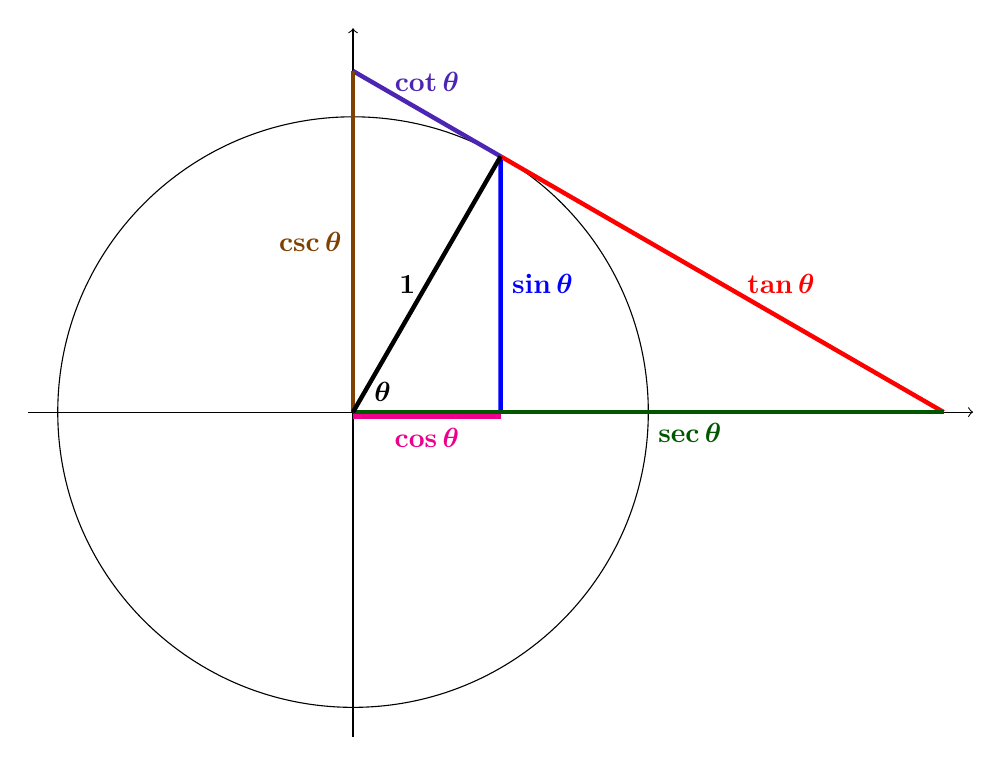
\begin{tikzpicture}[scale = 3.75]
    \draw [->, thin] (-1.1,0) -- (2.1,0);
    \draw [->, thin] (0,-1.1) -- (0,1.3);
    \draw (0,0) circle (1);
    \coordinate (A) at (0.5,0.86602540378);
    \boldmath
    \node at (.1,.07) {$\theta$};
    \draw [ultra thick, blue] (.5,0) to
    node [right] {$\sin \theta$} (A);
    \draw [ultra thick, red] (A) to
    node [right = 5] {$\tan \theta$} (2,0);
    \draw [ultra thick, black!66!green] (0,0) to
    node [below, xshift = 15] {$\sec \theta$} (2,0);
    \draw [ultra thick, magenta] (0,-.015) to
    node [below] {$\cos \theta$} (.5,-.015);
    \draw [ultra thick, orange!30!blue] (A) to
    node [above = 4] {$\cot \theta$} (0,1.155);
    \draw [ultra thick, black!50!orange] (0,0) to
    node [left] {$\csc \theta$} (0,1.155);
    \draw [ultra thick] (0,0) to node [left] {$1$} (A);
    \unboldmath
  \end{tikzpicture}
\end{center}


\end{document}
